\section{Système proie-prédateur de Lotka-Volterra}\label{sec:sec2}
Dans cette partie, nous allons étudier le système proie-prédateur de Lotka-Volterra,
qui est un système d'équations différentielles ordinaires,
et le comparer à des modèles plus simples.


\subsection{Modèles simplistes}
Un des premiers modèle de population est celui de Malthus, qui suppose une croissance exponentielle de la population $N(t)$.
Celui-ci utilise l'équation $\frac{dN(t)}{dt} = \gamma N(t)$, avec $\gamma \in \mathbb{R}$.

Un coefficient $\gamma$ positif implique une croissance de la population, et un coefficient négatif une décroissance.
Un autre modèle a été proposé, celui de Verhulst, utilisant une formule similaire à celle de Malthus,
à la différence qu'il ne croît pas au delà d'une certaine population $\kappa$, ce qui simule une limite de ressources.
Il utilise l'équation $\frac{dN(t)}{dt} = \gamma N(t) \left( 1 - \frac{N(t)}{\kappa} \right)$,
avec $N(t)$ la population à l'instant $t$ (à un facteur près), $\gamma \in \mathbb{R}$ et $\kappa \in \mathbb{R}$.

Les résultats de ces deux modèles sont présentés sur la figure~\ref{fig:populations}, ce qui montre bien que le modèle de Verhulst
est plus réaliste que celui de Malthus.

\begin{figure}[htbp!]
	\centering
	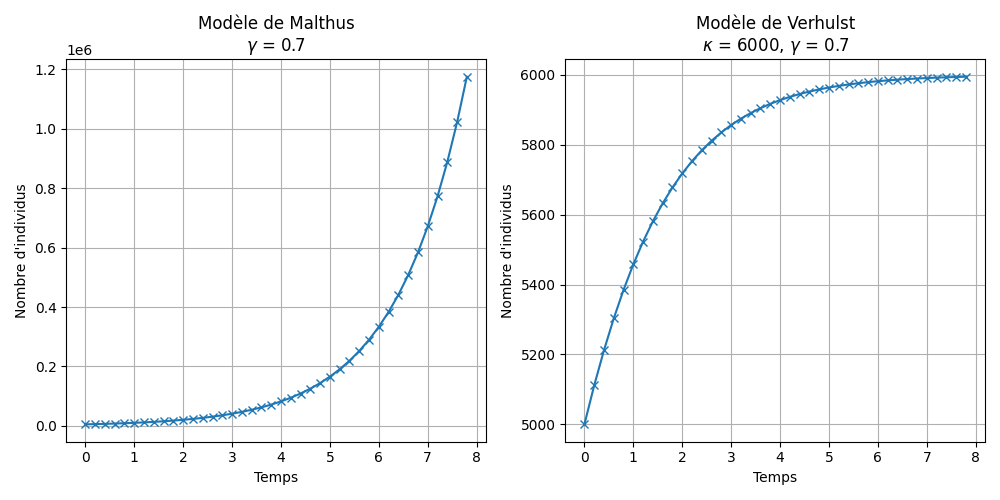
\includegraphics[width=0.7\textwidth]{res/population}
	\caption{Comparaison des modèles de Malthus et de Verhulst, avec initialement $40$ individus.}
	\label{fig:populations}
\end{figure}

Le modèle de Lotka-Volterra est un modèle plus réaliste, qui prend en compte deux populations,
l'une de proies, l'autre de prédateurs.
Il utilise les équations~\ref{eq:lotka}, avec $N(t)$ la population de proies à l'instant $t$ (à un facteur près),
$P(t)$ la population de prédateurs à l'instant $t$, $(a, b, c, d) \in (\mathbb{R}^{+*})^4$.

\begin{equation}
	\label{eq:lotka}
	\frac{dN(t)}{dt} = N(t) \times (a - b \times P(t)) \ \ \ \ \ \ \ \ \ \ \ \ \ \ \
	\frac{dP(t)}{dt} = P(t) \times (c \times N(t) - d)
\end{equation}

Après résolution avec \texttt{meth\_epsilon}, on obtient la figure~\ref{fig:lotka}, qui montre une solution périodique.

\begin{figure}[htbp!]
	\centering
	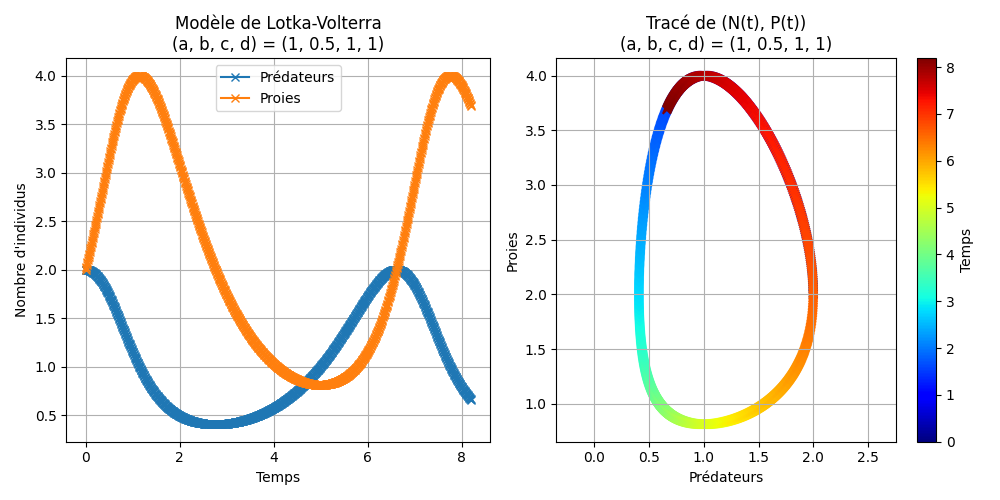
\includegraphics[width=0.7\textwidth]{res/lotka}
	\caption{Résolution du système de Lotka-Volterra, avec initialement $2$ proies et $2$ prédateurs.}
	\label{fig:lotka}
\end{figure}

De sorte à calculer rapidement la période des oscillations des deux populations, on itère
sur les valeurs échantillonnées, et on vérifie si la valeur actuelle est proche de la toute première.

Concernant les solutions constantes pour ce modèle, elles sont obtenues pour des dérivées nulles,
ce qui se traduit par la formule logique~\ref{eq:lotka-const}. Ce sont les points singuliers
de l'équation différentielle.

\begin{equation}
	\label{eq:lotka-const}
	\left(\left(N(t) = 0\right) \vee \left(P(t) = \frac{a}{b}\right)\right)
	\wedge
	\left(\left(P(t) = 0\right) \vee \left(N(t) = \frac{d}{c}\right)\right), \forall t \in \mathbb{R}
\end{equation}

En traçant les solutions proches d'un point non-singulier, on obtient la figure~\ref{fig:behaviour}. Systématiquement,
pour des points non-singuliers, on obtient des solutions périodiques, et donc un cycle fermé, de forme déterminée par les paramètres.
Pour des points singuliers, on a des ellipses si les valeurs ne sont pas nulles, selon la formule~\ref{eq:lotka-const},
et des droites si l'une des valeurs est nulle, sinon un point.

\begin{figure}[htbp!]
	\centering
	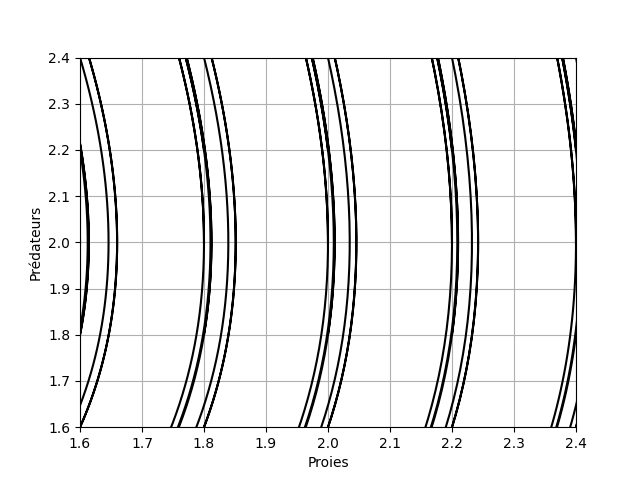
\includegraphics[width=0.45\textwidth]{res/behaviour}
	\caption{Comportement des solutions proches d'un point non-singulier (rectangle autour de $(2, 2)$)}
	\label{fig:behaviour}
\end{figure}

Dans le cas général, pour une équation différentielle quelconque, il n'y a pas nécessairement de cycle fermé dans une représentation
telle que celle de la figure~\ref{fig:behaviour}.
